\chapter{Risultati} \label{chp:risultati}
Nel seguente capitolo verranno presentati e discussi i risultati ottenuti dai
modelli precedentemente addestrati. I risultati sono stati ottenuti attraverso
due metodologie di valutazione:
\begin{enumerate}
    \item \textbf{Valutazione $80/20$}: i modelli sono stati allenati su un
          training set e valutati su un test set, entrambi estratti dal dataset
          originale.
    \item \textbf{Valutazione con $10$-fold cross-validation}: i modelli sono
          stati allenati e valutati su $10$ partizioni del dataset originale in
          modo da ottenere una stima più accurata delle performance del modello.
\end{enumerate}
I classificatori sono stati valutati calcolando la matrice di confusione e le
seguenti metriche:
\begin{itemize}
    \item \textbf{Accuracy}
    \item \textbf{Precision}
    \item \textbf{Recall}
    \item \textbf{F1-score}
\end{itemize}

In aggiunta, sono state calcolate le curve ROC per analizzare True Positive rate
e False Positive rate.

Durante la seconda fase di valutazione dei modelli sono state calcolate le
metriche precedentemente specificate e per ciascun di esse gli intervalli di
confidenza.
\section{Risultati dataset correlazione} \label{sec:risultati_corr}
Come precedentemente specificato, i modelli sono stati addestrati su due dataset.
In questa sezione verranno presentati i risultati ottenuti dai modelli addestrati
sul dataset ricavato tramite riduzione attraverso correlazione delle feature.
\subsection*{Valutazione $80/20$}
Il primo studio condotto consiste nella suddivisione del dataset in training
set e test set. Questa suddivisione ha permesso di calcolare le performance dei
modelli e confrontarli.

In primo luogo, sono state generate le matrici di confusione per ciascun
modello, le quali sono illustrate nella figura \ref{fig:matrice_di_confusione_per_corr}.
\begin{figure}[!ht]
    \centering
    \begin{subfigure}{0.3\textwidth}
        \centering
        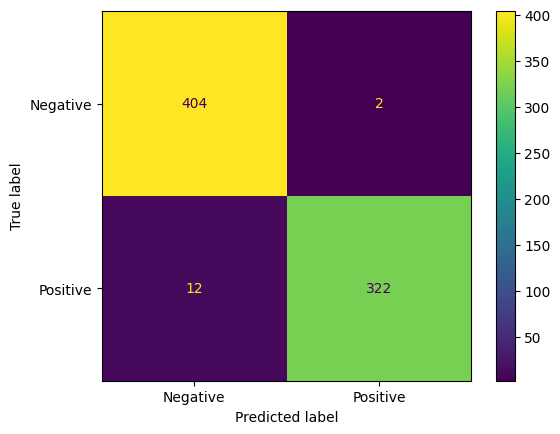
\includegraphics[width=\textwidth]{img/svm/matrice_confusione_corr.png}
        \caption{Support Vector Machine}
        \label{fig:matrice_di_confusione_per_SVM_corr}
    \end{subfigure}
    \hfill
    \begin{subfigure}{.3\textwidth}
        \centering
        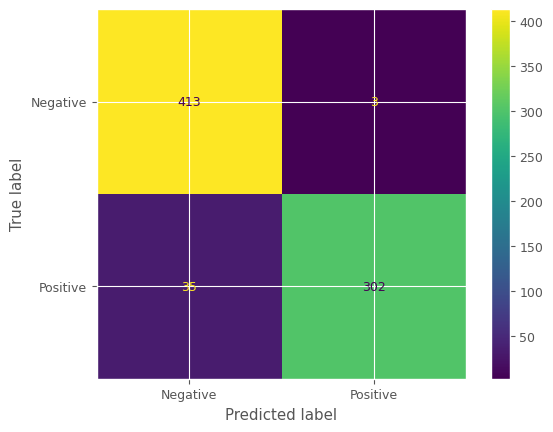
\includegraphics[width=\textwidth]{img/gnb/confusion_matrix_corr.png}
        \caption{Gaussian Naive Bayes}
        \label{fig:matrice_di_confusione_per_GNB_corr}
    \end{subfigure}
    \hfill
    \begin{subfigure}{.3\textwidth}
        \centering
        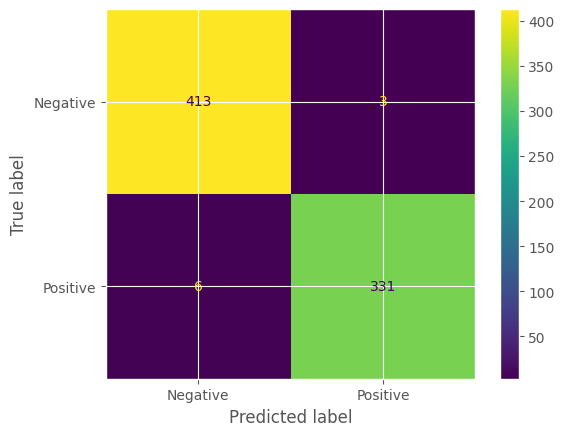
\includegraphics[width=\textwidth]{img/rete/matrice_confusione.png}
        \caption{Rete neurale}
        \label{fig:matrice_di_confusione_per_NN_corr}
    \end{subfigure}
    \caption{Matrici di confusione per i modelli addestrati su \texttt{dataset\_corr} e \texttt{dataset\_corr\_std}}
    \label{fig:matrice_di_confusione_per_corr}
\end{figure}

Le matrici di confusione evidenziano che i tre modelli presentano una buona
capacità di discriminazione tra le due classi, come dimostrato dal numero
elevato di veri positivi e veri negativi. In particolare, sia il modello SVM che
la rete neurale mostrano performance identiche, mentre il modello Gaussian Naive
Bayes è caratterizzato da un numero maggiore di errori.

Si osserva una tendenza comune a commettere più errori nella classificazione
degli esempi di falsi negativi rispetto a falsi positivi per tutti i modelli.
Questo fenomeno potrebbe essere spiegato da un leggero sbilanciamento del dataset
verso la classe negativa.

Dalle matrici di confusione si sono successivamente ricavate le metriche
precedentemente specificate. Nella tabella \ref{tab:risultati}, sono riportate
le performance dei modelli, calcolate sul test set.
\begin{table}[!ht]
    \centering
    \begin{tabular}{@{}clllll@{}}
        \toprule
        \rowcolor[HTML]{EFEFEF}
        \textbf{Modello}                                      & \textbf{Accuracy}            & \textbf{Precision}           & \textbf{Recall}              & \textbf{F1-score}            & \textbf{Tempo}              \\ \midrule
        \cellcolor[HTML]{EFEFEF}\textbf{SVM}                  & \multicolumn{1}{c}{98.10 \%} & \multicolumn{1}{c}{99.38 \%} & \multicolumn{1}{c}{96.40 \%} & \multicolumn{1}{c}{97.87 \%} & \multicolumn{1}{c}{0.216 s} \\
        \cellcolor[HTML]{EFEFEF}\textbf{Gaussian Naive Bayes} & \multicolumn{1}{c}{94.05 \%} & \multicolumn{1}{c}{98.98 \%} & \multicolumn{1}{c}{87.87 \%} & \multicolumn{1}{c}{93.01 \%} & \multicolumn{1}{c}{0.006 s} \\
        \cellcolor[HTML]{EFEFEF}\textbf{Rete neurale}         & \multicolumn{1}{c}{97.83 \%} & \multicolumn{1}{c}{99.37 \%} & \multicolumn{1}{c}{95.80 \%} & \multicolumn{1}{c}{97.56 \%} & \multicolumn{1}{c}{6.681 s} \\ \bottomrule
    \end{tabular}
    \caption{Risultati ottenuti dal modello addestrato}
    \label{tab:risultati}
\end{table}

Dai risultati ottenuti si può evincere che la rete neurale e la Support Vector
Machine (SVM) hanno ottenuto performance elevate ma non evidenziando
una netta superiorità di uno dei due modelli, mentre il modello Gaussian
Naive Bayes ha mostrato performance leggermente inferiori. Tale fenomeno potrebbe
essere giustificato considerando che nel dataset sono presenti feature che non
rispettano la distribuzione gaussiana, quindi dal momento che si calcola la
verosimiglianza utilizzando la formula della distribuzione normale, Gaussian
Naive Bayes risulta più sensibile alla sua assunzione. Inoltre, la rete neurale
e SVM sono modelli intrinsecamente più complessi rispetto al Gaussian Naive
Bayes, consentendo loro di catturare relazioni più intricate tra le features e
la variabile target.

Questi risultati devono anche essere interpretati considerando che il tempo di
addestramento. Con questa premessa possiamo affermare che la SVM permette di
ottenere il miglior compromesso tra il tempo di addestramento e le performance
del modello.

In seguito, si è deciso di confrontare i modelli utilizzando le curve ROC con
le relative aree sottese (AUC), le quali permettono di confrontare i modelli in
termini di trade-off tra tasso di veri positivi e tasso di falsi positivi. In
aggiunta, queste curve confrontano i modelli indipendentemente dal valore di
soglia utilizzato per la classificazione, il che permette di evitare la fase di
ottimizzazione del modello rispetto ad una particolare soglia.

Per avere un modello di confronto si è deciso di aggiungere al grafico delle
curve ROC anche quella di un classificatore randomico. Le curve ROC del
classificatore casuale e dei tre modelli allenati sono visibili nella figura
\ref{fig:roc_curve_corr}.
\begin{figure}[!ht]
    \centering
    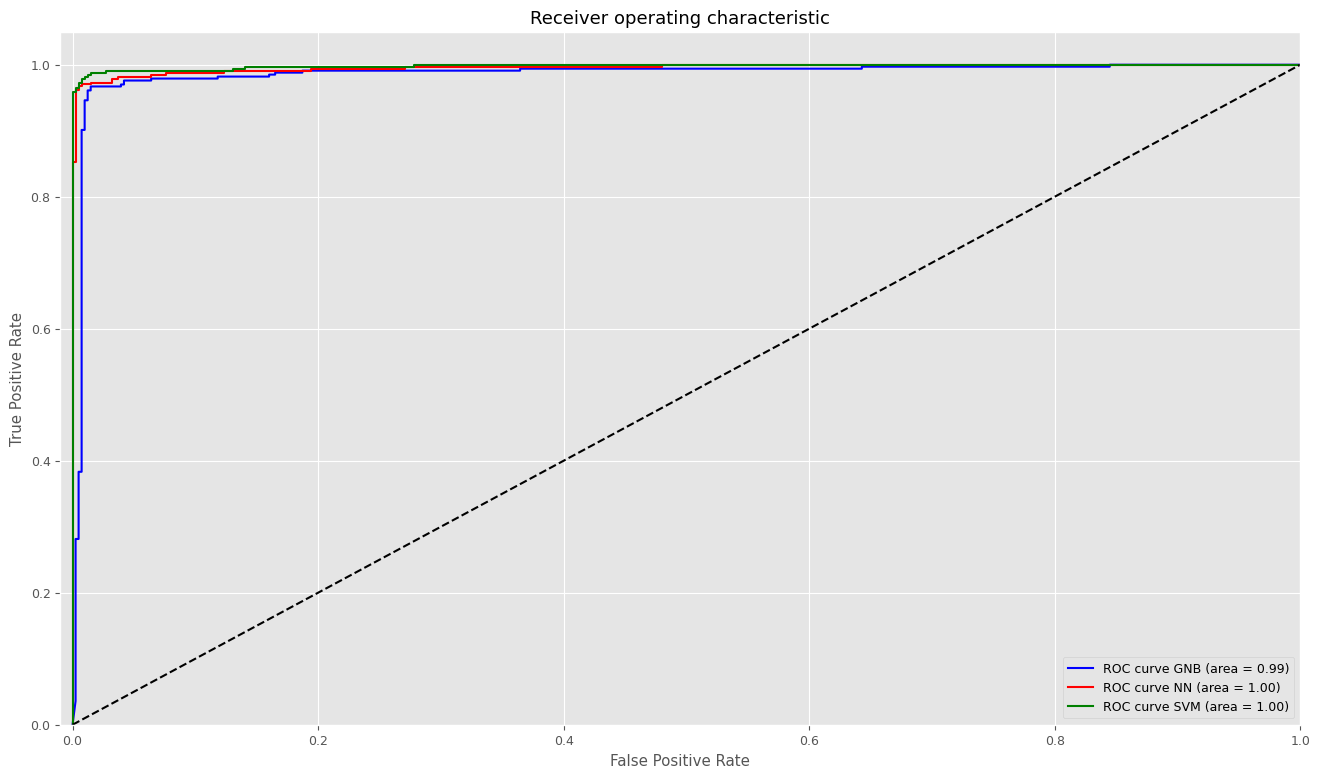
\includegraphics[width=\textwidth]{img/ris/roc_curve_corr.png}
    \caption{Curve ROC per i modelli addestrati su \texttt{dataset\_corr} e \texttt{dataset\_corr\_std}}
    \label{fig:roc_curve_corr}
\end{figure}

Il grafico rappresentato nella figura \ref{fig:roc_curve_corr} evidenzia che i
tre modelli addestrati mostrano prestazioni molto simili tra loro e
significativamente migliori rispetto al classificatore casuale. Pertanto, risulta
cruciale concentrarsi sul confronto dell'area sotto la curva ROC (AUC). L'area
sotto la curva ROC per la rete neurale e per SVM è pari a $1.00$, mentre per il
Gaussian Naive Bayes è pari a $0.99$. Questi valori non consentono di stabilire
una netta superiorità di uno dei tre modelli, ma suggeriscono che i modelli di
rete neurale e SVM siano leggermente superiori al Gaussian Naive Bayes.
\subsection*{Valutazione con $10$-fold cross-validation}
Il secondo studio condotto consiste nel valutare i modelli attraverso la tecnica
della $10$-fold stratified cross-validation. Questa tecnica permette di ottenere
una stima più accurata delle performance del modello, riducendo l'effetto della
variabilità dei dati.

In questo processo, per ogni modello addestrato sono state calcolate nuovamente
le metriche specificate nell'introduzione del capitolo. I risultati ottenuti
dall'esecuzione della cross-validation sono stati successivamente utilizzati per
calcolare gli intervalli di confidenza al $90\%$ delle metriche sopracitate.

Per svolgere questa operazione sono stati utilizzati \texttt{dataset\_corr} e
\texttt{dataset\_corr\_std} senza alcuna suddivisione in training set e test set,
dal momento che le separazioni vengono effettuate all'interno della $10$-fold.

I risultati ottenuti sono stati riportati nella tabella \ref{tab:intervalli_confidenza_corr}
e che grafica in figura \ref{fig:img_intervalli_confidenza_corr}.
\begin{table}[!ht]
    \begin{subtable}[h]{1\textwidth}
        \centering
        \begin{tabular}{@{}clllll@{}}
            \toprule
            \rowcolor[HTML]{EFEFEF}
            \textbf{Modello}                                      & \textbf{Accuracy}            & \textbf{Precision}           & \textbf{Recall}              & \textbf{F1-score}            & \textbf{Tempo}              \\ \midrule
            \cellcolor[HTML]{EFEFEF}\textbf{SVM}                  & \multicolumn{1}{c}{98.10 \%} & \multicolumn{1}{c}{99.38 \%} & \multicolumn{1}{c}{96.40 \%} & \multicolumn{1}{c}{97.87 \%} & \multicolumn{1}{c}{0.216 s} \\
            \cellcolor[HTML]{EFEFEF}\textbf{Gaussian Naive Bayes} & \multicolumn{1}{c}{94.05 \%} & \multicolumn{1}{c}{98.98 \%} & \multicolumn{1}{c}{87.87 \%} & \multicolumn{1}{c}{93.01 \%} & \multicolumn{1}{c}{0.006 s} \\
            \cellcolor[HTML]{EFEFEF}\textbf{Rete neurale}         & \multicolumn{1}{c}{98.35 \%} & \multicolumn{1}{c}{98.79 \%} & \multicolumn{1}{c}{97.54 \%} & \multicolumn{1}{c}{98.16 \%} & \multicolumn{1}{c}{?? s}    \\ \bottomrule
        \end{tabular}
        \caption{Valore medio delle metriche ottenute dalla cross validation}
        \label{tab:risultati_cross_val_corr}
    \end{subtable}
    \hfill
    \begin{subtable}[h]{1\textwidth}
        \centering
        \begin{tabular}{@{}cllll@{}}
            \toprule
            \rowcolor[HTML]{EFEFEF}
            \textbf{Modello}                                      & \textbf{Accuracy}  & \textbf{Precision} & \textbf{Recall}    & \textbf{F1-score}  \\ \midrule
            \cellcolor[HTML]{EFEFEF}\textbf{SVM}                  & [98.71\%, 99.45\%] & [99.17\%, 99.98\%] & [97.68\%, 99.07\%] & [98.55\%, 99.39\%] \\
            \cellcolor[HTML]{EFEFEF}\textbf{Gaussian Naive Bayes} & [94.85\%, 95.84\%] & [98.76\%, 99.40\%] & [89.49\%, 91.59\%] & [94.01\%, 95.21\%] \\
            \cellcolor[HTML]{EFEFEF}\textbf{Rete neurale}         & [97.90\%, 98.80\%] & [98.35\%, 99.23\%] & [96.81\%, 98.29\%] & [97.66\%, 98.66\%] \\ \bottomrule
        \end{tabular}
        \caption{Intervalli di confidenza delle metriche ottenute dalla cross validation}
        \label{tab:intervalli_confidenza_corr}
    \end{subtable}
    \caption{Risultati ottenuti dalla cross validation}
    \label{tab:metriche_intervalli_confidenza_corr}
\end{table}

\begin{figure}[!ht]
    \centering
    \begin{subfigure}[b]{0.4\textwidth}
        \centering
        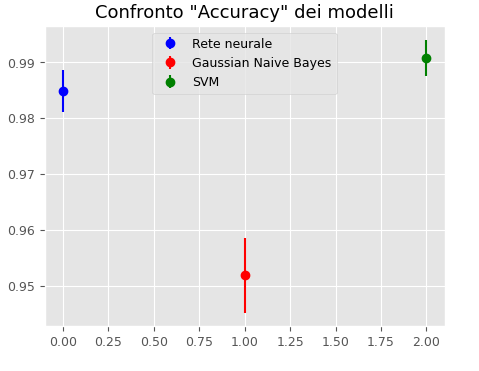
\includegraphics[width=\textwidth]{img/ris/accuracy_inter_corr.png}
        \caption{Accuracy}
        \label{fig:acc}
    \end{subfigure}
    \hfill
    \begin{subfigure}[b]{0.4\textwidth}
        \centering
        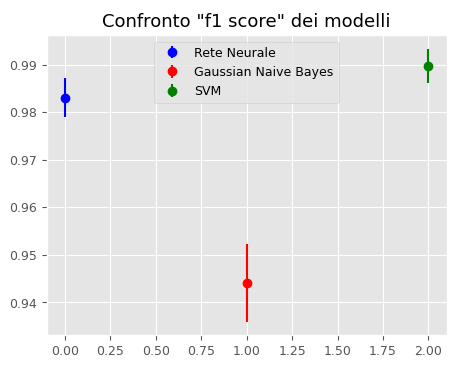
\includegraphics[width=\textwidth]{img/ris/fscore_inter_corr.png}
        \caption{F1 score}
        \label{fig:f1}
    \end{subfigure}
    \hfill
    \begin{subfigure}[b]{0.4\textwidth}
        \centering
        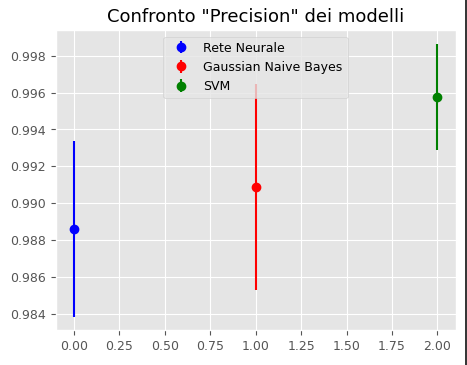
\includegraphics[width=\textwidth]{img/ris/precision_inter_corr.png}
        \caption{Precision}
        \label{fig:precision}
    \end{subfigure}
    \hfill
    \begin{subfigure}[b]{0.4\textwidth}
        \centering
        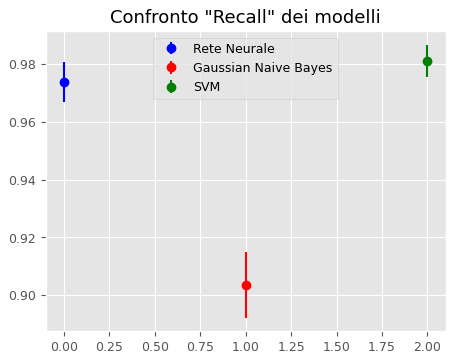
\includegraphics[width=\textwidth]{img/ris/recall_inter_corr.png}
        \caption{Recall}
        \label{fig:recall}
    \end{subfigure}
    \caption{Intervalli di confidenza ottenuti dai modelli addestrati con e senza PCA}
    \label{fig:img_intervalli_confidenza_corr}
\end{figure}

Dagli intervalli di confidenza si nota immediatamente che Gaussian Naive Bayes è
il peggiore rispetto agli altri modelli secondo le metriche di Accuracy, Recall
e F1-score, non solo in termini di media degli intervalli, ma anche in termini
di varianza delle metriche. Questo significa che tra tutti i modelli allenati
sulla versione del dataset con le feature selezionate tramite correlazione, i
migliori sono rete neurale e SVM, più precisamente si hanno risultati migliori
del circa $4\%-8\%$ sulle metriche rispetto a Gaussian Naive Bayes. Al contrario
la Precision risulta simile tra i modelli.
\newpage
\section{Risultati dataset PCA} \label{sec:risultati_pca}
Un ragionamento analogo a quello svolto nella sezione \ref{sec:risultati_corr}
può essere applicato ai modelli addestrati sul dataset le cui feature sono state
calcolate attraverso Principal Component Analysis (PCA).
\subsection*{Valutazione $80/20$}
Il primo studio condotto consiste nella suddivisione del dataset in training
set e test set. Questa suddivisione ha permesso di calcolare le performance dei
modelli e confrontarli.

In primo luogo, sono state generate le matrici di confusione per ciascun
modello, le quali sono illustrate nella figura \ref{fig:matrice_di_confusione_per_pca}.
\begin{figure}[!ht]
    \centering
    \begin{subfigure}{.3\textwidth}
        \centering
        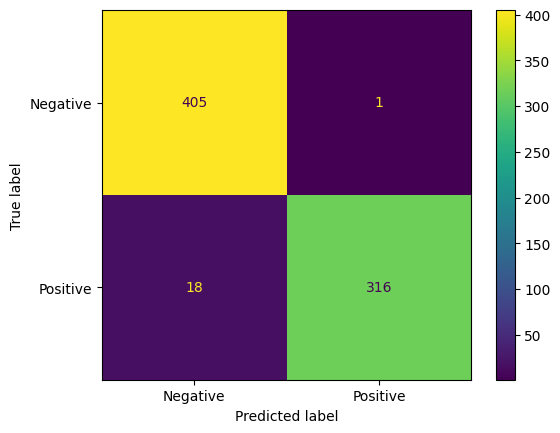
\includegraphics[width=\textwidth]{img/svm/matrice_confusione_pca.png}
        \caption{Support Vector Machine}
        \label{fig:matrice_di_confusione_per_SVM_pca}
    \end{subfigure}
    \hfill
    \begin{subfigure}{.3\textwidth}
        \centering
        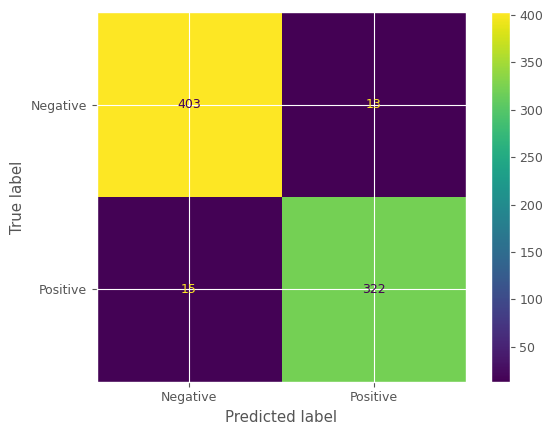
\includegraphics[width=\textwidth]{img/gnb/confusion_matrix_pca.png}
        \caption{Gaussian Naive Bayes}
        \label{fig:matrice_di_confusione_per_GNB_pca}
    \end{subfigure}
    \hfill
    \begin{subfigure}{.3\textwidth}
        \centering
        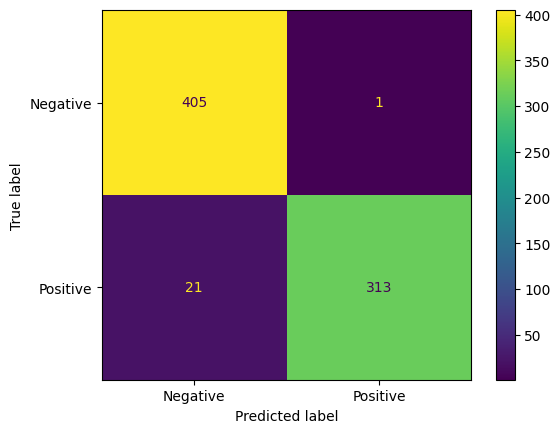
\includegraphics[width=\textwidth]{img/rete/matrice_confusione_PCA.png}
        \caption{Rete neurale}
        \label{fig:matrice_di_confusione_per_NN_pca}
    \end{subfigure}
    \caption{Matrici di confusione per i modelli addestrati su \texttt{dataset\_pca} e \texttt{dataset\_pca\_std}}
    \label{fig:matrice_di_confusione_per_pca}
\end{figure}

In questo caso si può notare come SVM e la rete neurale presentino un numero
maggiore di errori rispetto ai modelli precedentemente analizzati. In particolare,
il numero di falsi negativi è simile tra i tre modelli, mentre il numero di falsi
positivi è minore per SVM e la rete neurale rispetto a Gaussian Naive Bayes.

Come fatto in precedenza, sono state ricavate dalle matrici di confusione le
metriche per calcolare le performance dei modelli. I risultati ottenuti sono stati
riportati nella tabella \ref{tab:risultati_pca}.
\begin{table}[!ht]
    \centering
    \begin{tabular}{@{}clllll@{}}
        \toprule
        \rowcolor[HTML]{EFEFEF}
        \textbf{Modello}                                      & \textbf{Accuracy}            & \textbf{Precision}           & \textbf{Recall}              & \textbf{F1-score}            & \textbf{Tempo}              \\ \midrule
        \cellcolor[HTML]{EFEFEF}\textbf{SVM}                  & \multicolumn{1}{c}{97.43 \%} & \multicolumn{1}{c}{100.0 \%} & \multicolumn{1}{c}{94.31 \%} & \multicolumn{1}{c}{97.07 \%} & \multicolumn{1}{c}{0.196 s} \\
        \cellcolor[HTML]{EFEFEF}\textbf{Gaussian Naive Bayes} & \multicolumn{1}{c}{95.41 \%} & \multicolumn{1}{c}{95.73 \%} & \multicolumn{1}{c}{94.01 \%} & \multicolumn{1}{c}{94.86 \%} & \multicolumn{1}{c}{0.006 s} \\
        \cellcolor[HTML]{EFEFEF}\textbf{Rete neurale}         & \multicolumn{1}{c}{97.16 \%} & \multicolumn{1}{c}{99.68 \%} & \multicolumn{1}{c}{94.01 \%} & \multicolumn{1}{c}{96.76 \%} & \multicolumn{1}{c}{2.226 s} \\ \bottomrule
    \end{tabular}
    \caption{Risultati ottenuti dal modello addestrato}
    \label{tab:risultati_pca}
\end{table}

I risultati ottenuti evidenziano un lieve peggioramento delle performance
rispetto ai modelli precedentemente analizzati. Un vantaggio dell'utilizzo di
PCA è dovuto al fatto che avendo ridotto il numero di feature a $3$, il tempo di
addestramento dei modelli è diminuito.

Questo ci suggerisce che la sua applicazione potrebbe essere un operazione
non risulta essere vantaggiosa. Questo risultato deve essere ulteriormente
verificato attraverso l'analisi delle curve ROC e il processo di valutazione
attraverso la cross-validation.

Nello specifico, dalle curve ROC create per i modelli addestrati sul dataset
estratto con PCA (vedi figura \ref{fig:roc_curve_pca}), si nota una maggiore
distanza tra la rete neurale e la SVM rispetto a quella del Bayes.
Questo si può osservare principalmente nella parte sinistra del grafico, dove si
ha un tasso di falsi positivi molto basso.

\begin{figure}[!ht]
    \centering
    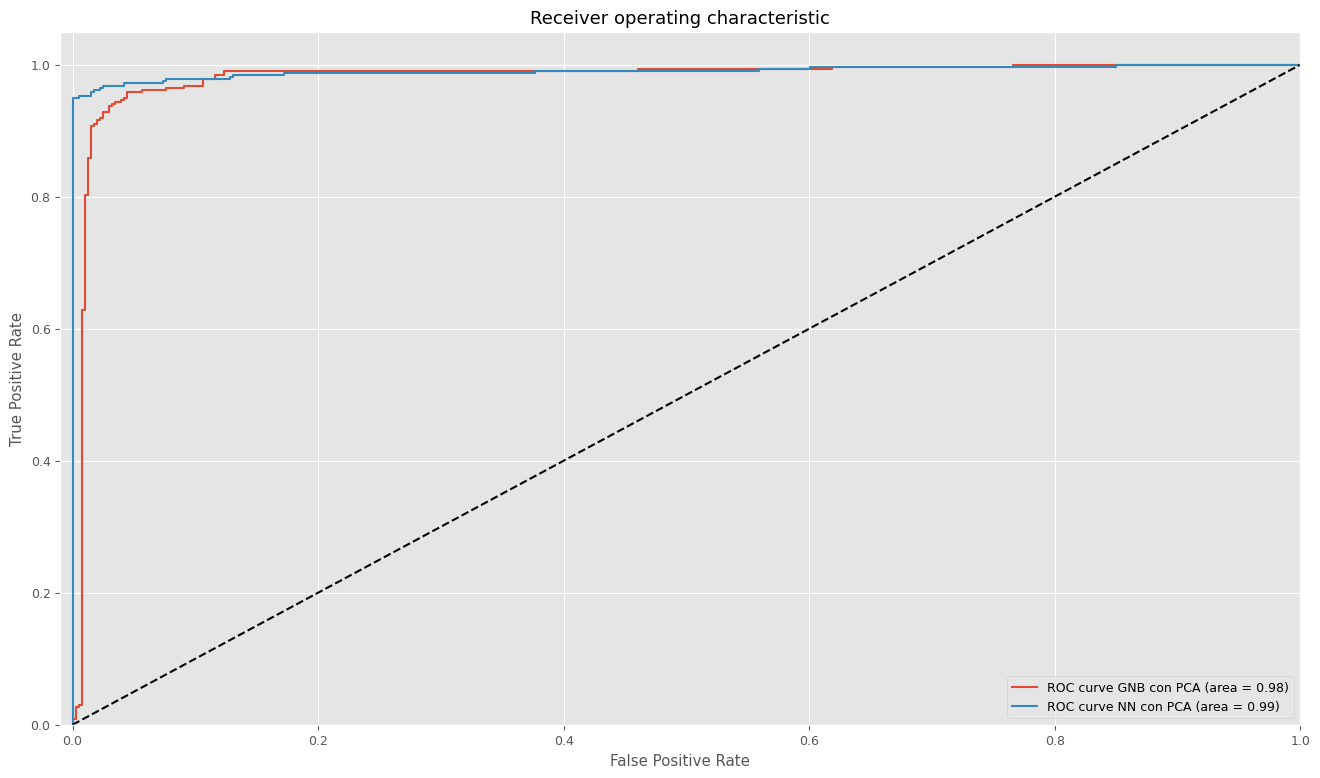
\includegraphics[width=\textwidth]{img/ris/roc_curve_pca.png}
    \caption{Curve ROC per i modelli addestrati su \texttt{dataset\_pca} e \texttt{dataset\_pca\_std}}
    \label{fig:roc_curve_pca}
\end{figure}

Come osservato anche nell'analisi delle curve ROC svolta in precedenza, i tre
modelli addestrati mostrano prestazioni molto simili tra loro e significativamente
migliori rispetto al classificatore casuale. Data la somiglianza delle curve ROC,
è necessario confrontare i modelli in termini di area sottesa alla curva ROC (AUC).
L'area sottesa alla curva ROC per la rete neurale e della SVM sono pari a $0.99$,
mentre per il Gaussian Naive Bayes è pari a $0.98$.

Questi valori suggeriscono, come per la sezione precedente, che la SVM e la rete
siano leggermente superiori a Bayes in termini di capacità discriminante tra le
classi.
\subsection*{Valutazione con $10$-fold cross-validation}
Per concludere, è stata effettuata la valutazione attraverso $10$-fold
cross-validation. I risultati ottenuti sono stati riportati in figura
\ref{fig:intervalli_confidenza_pca} e nella tabella \ref{tab:intervalli_confidenza_pca}.
\begin{table}[!ht]
    \begin{subtable}[h]{1\textwidth}
        \centering
        \begin{tabular}{@{}cllll@{}}
            \toprule
            \rowcolor[HTML]{EFEFEF}
            \textbf{Modello}                                      & \textbf{Accuratezza}         & \textbf{Precisione}          & \textbf{Richiamo}            & \textbf{F1 score}            \\ \midrule
            \cellcolor[HTML]{EFEFEF}\textbf{SVM}                  & \multicolumn{1}{c}{99.05 \%} & \multicolumn{1}{c}{99.57 \%} & \multicolumn{1}{c}{98.32 \%} & \multicolumn{1}{c}{98.94 \%} \\
            \cellcolor[HTML]{EFEFEF}\textbf{Gaussian Naive Bayes} & \multicolumn{1}{c}{96 \%}    & \multicolumn{1}{c}{96 \%}    & \multicolumn{1}{c}{96 \%}    & \multicolumn{1}{c}{96 \%}    \\
            \cellcolor[HTML]{EFEFEF}\textbf{Rete neurale}         & \multicolumn{1}{c}{98.35 \%} & \multicolumn{1}{c}{98.73 \%} & \multicolumn{1}{c}{97.61 \%} & \multicolumn{1}{c}{98.16 \%} \\ \bottomrule
        \end{tabular}
        \caption{Valore medio delle metriche ottenute dalla cross validation}
        \label{tab:risultati_cross_val_pca}
    \end{subtable}
    \hfill
    \begin{subtable}[h]{1\textwidth}
        \centering
        \begin{tabular}{@{}cllll@{}}
            \toprule
            \rowcolor[HTML]{EFEFEF}
            \textbf{Modello}                                      & \textbf{Accuratezza} & \textbf{Precisione} & \textbf{Richiamo}  & \textbf{F1 score}  \\ \midrule
            \cellcolor[HTML]{EFEFEF}\textbf{SVM}                  & [98.75\%, 99.35\%]   & [99.34\%, 99.81\%]  & [97.65\%, 98.99\%] & [98.60\%, 99.27\%] \\
            \cellcolor[HTML]{EFEFEF}\textbf{Gaussian Naive Bayes} & [94.73\%, 95.85\%]   & [98.65\%, 99.53\%]  & [89.14\%, 91.70\%] & [93.85\%, 95.22\%] \\
            \cellcolor[HTML]{EFEFEF}\textbf{Rete neurale}         & [97.93\%, 98.77\%]   & [98.29\%, 99.18\%]  & [96.87\%, 98.33\%] & [97.69\%, 98.63\%] \\ \bottomrule
        \end{tabular}
        \caption{Intervalli di confidenza delle metriche ottenute dalla cross validation}
        \label{tab:intervalli_confidenza_pca}
    \end{subtable}
    \caption{Risultati ottenuti dalla cross validation}
    \label{tab:media_intervalli_confidenza_pca}
\end{table}

Analizzando i risultati della cross-validation, si ha una conferma che SVM e
rete neurale mostrano performance superiori rispetto a Bayes. In particolare,
SVM è il modello che mostra le performance migliori sia in termini di media delle
metriche, sia in termini di varianza delle stesse.

A differenza di quanto osservato nel dataset le cui feature sono state selezionate
tramite studio della correlazione, in questo caso l'applicazione di PCA non
porta significativi incrementi alle performance.

L'unica differenza si riscontra nel caso di Gaussian Naive Bayes, il quale ha
avuto un decremento della media delle metriche e un aumento dell'ampiezza degli
intervalli di confidenza, suggerendo una perdita di robustezza.
\begin{figure}[!ht]
    \centering
    \begin{subfigure}[b]{0.4\textwidth}
        \centering
        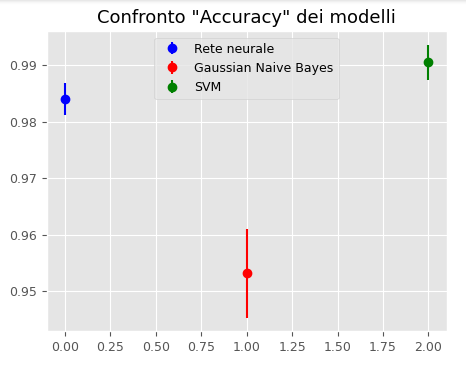
\includegraphics[width=\textwidth]{img/ris/accuracy_inter_pca.png}
        \caption{Accuracy}
        \label{fig:acc_pca}
    \end{subfigure}
    \hfill
    \begin{subfigure}[b]{0.4\textwidth}
        \centering
        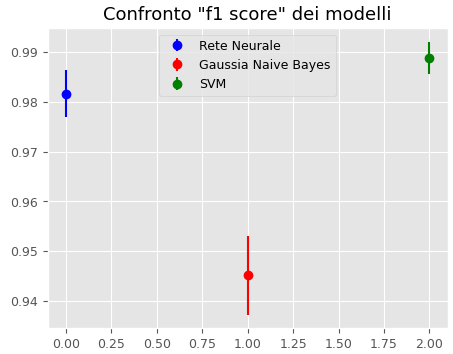
\includegraphics[width=\textwidth]{img/ris/fscore_inter_pca.png}
        \caption{F1 score}
        \label{fig:f1_pca}
    \end{subfigure}
    \hfill
    \begin{subfigure}[b]{0.4\textwidth}
        \centering
        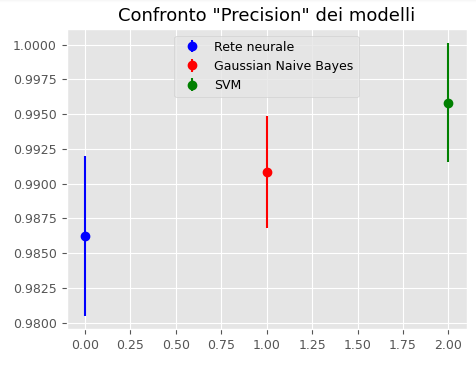
\includegraphics[width=\textwidth]{img/ris/precision_inter_pca.png}
        \caption{Precision}
        \label{fig:precision_pca}
    \end{subfigure}
    \hfill
    \begin{subfigure}[b]{0.4\textwidth}
        \centering
        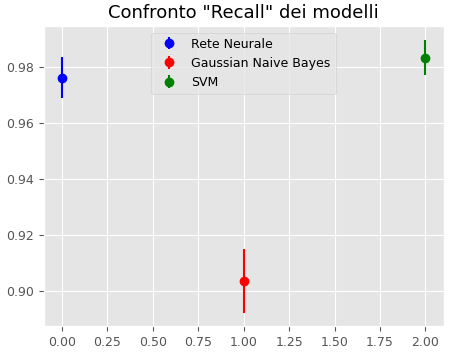
\includegraphics[width=\textwidth]{img/ris/recall_inter_pca.png}
        \caption{Recall}
        \label{fig:recall_pca}
    \end{subfigure}
    \caption{Intervalli di confidenza ottenuti dai modelli addestrati con e senza PCA}
    \label{fig:intervalli_confidenza_pca}
\end{figure}

Questo studio permette di affermare che l'applicazione di PCA non ha portato a
miglioramenti significativi nelle performance dei modelli.